
\subsection{Sparse Distributed Representation}
% \subsection{The Datastructure of the Brain}


\begin{frame}[c,fragile]{Data Saving - Computer Science Solution}
    \Large
    What is \verb|01100101|? \pause Could be either one of:
    % What is ? Could be:
    \begin{itemize}[<+(1)->]
        \item Booleans (\verb|False, True, True, False,|\dots)
        \item Integer (\verb|101|)
        \item Float (\verb|3328|)
        \item (Byte-) String (\verb|'e'|)
        \item Pointer to something else
        \item Part of some other Datastructure
    \end{itemize}
\end{frame}

% \begin{frame}[c]{Primitive Computer Science Data Formats}
%     \Large
%     \begin{itemize}[<+(1)->]
%         \item Boolean
%         \item Integer
%         \item Float
%         \item (Byte-) String
%     \end{itemize}
% 
%     \vspace{0.5cm}
% 
%     \pause
% 
%     $\rightarrow$ Data is clearly seperated from Encoding, Meaning comes from actual Encoding
% \end{frame}


\begin{frame}[standout]
    \Large
    Biologically, this does not work out.

    \pause
    We use only 10\% of our Brain, right?
\end{frame}


\begin{frame}[c]{Sparse Distributed Representation - Example}
    \pause
    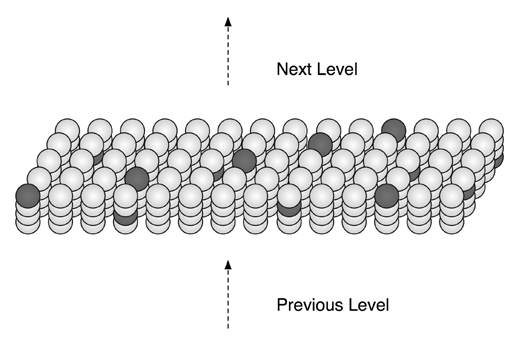
\includegraphics[width=0.95\textwidth]{region_sparse}
    % 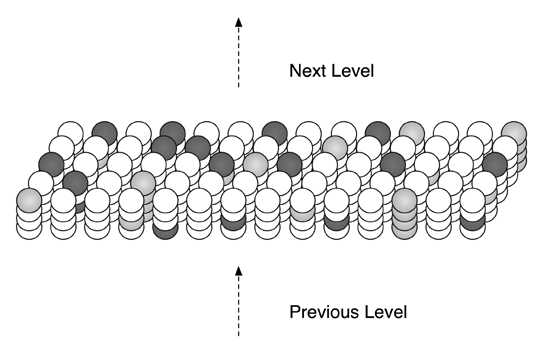
\includegraphics[width=0.9\textwidth]{region_predict}
\end{frame}


\begin{frame}[c]{Sparse Distributed Representation - Introduction}
    \Large
    \begin{itemize}[<+(1)->]
        \item Datastructure of the Brain
        \item Sparse (around 2\% are active)
        \item Distributed (clusters are somewhat rare)
        \item Inhibitory Mechanisms
        \item Neuron States actually have 'Meaning'
    \end{itemize}
\end{frame}





% \begin{frame}[c]{Bit Arrays}
%     \Large
%     \pause
%     % Who can code ... ?
% \end{frame}


% \begin{frame}[c]{Attributes of the Brain}
%     \Large
%     \begin{itemize}[<+(1)->]
%         \item Invariant
%         \item Auto-associative
%         \item Massively Parallel
%     \end{itemize}
% \end{frame}



